\chapter{Architecture}

\begin{figure}[H]
	\centering
	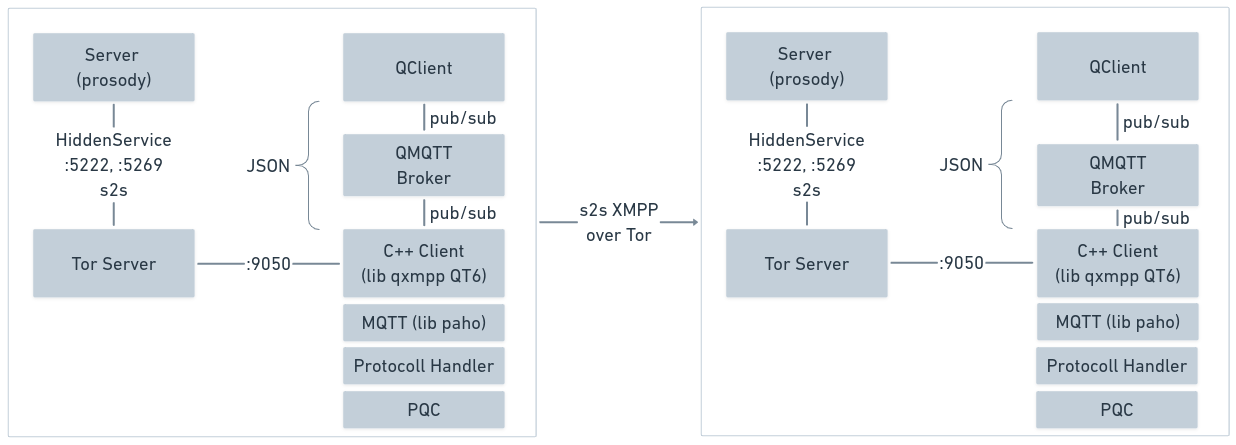
\includegraphics[width=1\linewidth]{resources/architecture.png}
	\caption{Architecture}
	\label{fig:architecture}
\end{figure}

\section {Client Design Decisions}

In the following chapters, we'll look in detail at the design and technology choices we've made, and consider their advantages and disadvantages.
Our primary focus is on secure and anonymous peer-to-peer communication. To achieve this we have thoroughly evaluated the following key topics.

\subsection{P2P Protocol}
\label{sec:p2pprotocol}
Initially, we looked at different peer-to-peer (P2P) protocols and finally focused on two: Matrix \cite{matrix2023website} and XMPP \cite{xmpp2023website}.


\subsubsection*{Protocol Comparison}

\textbf{XMPP Advantages}
\begin{itemize}
\item Customizable Server Settings: XMPP offers extensive configuration options, which provides flexibility in server setup, a significant advantage for specific use cases and environments.
\item Lightweight: Being more resource-efficient, XMPP uses less computational power and memory, leading to better performance, especially on limited-resource devices.
\item Available Server Software: The existence of several XMPP server software options like ejabberd and Prosody simplifies the implementation process, making it easier to deploy and manage.
\end{itemize}

\textbf{XMPP Disadvantages}
\begin{itemize}
\item Limited Metadata Privacy: Unlike Matrix, XMPP doesn’t inherently share conversation metadata across servers, but privacy concerns can still arise based on server configurations and client implementations.
\item Complex Federations: While XMPP supports server federations, managing these federations and ensuring interoperability and security across different servers can be complex.
\item Feature Set and Modernity: XMPP, being older, might not be as feature-rich or may require additional extensions for modern communication features compared to Matrix.
\end{itemize}

\textbf{Matrix Advantages}
\begin{itemize}
\item Rich Feature Set: Matrix is designed to support a wide range of modern communication features including VoIP, video calls, and more, making it suitable for versatile applications.
\item Federation and Decentralization: Matrix supports decentralized operation and federation, enabling users on different servers to communicate seamlessly.
\item Strong Metadata Sharing: Matrix shares conversation metadata across all servers, which can be beneficial for creating a unified and connected user experience.
\end{itemize}

\textbf{Matrix Disadvantages}
\begin{itemize}

\item Resource Intensive: Matrix can be more demanding in terms of computational resources compared to XMPP, potentially impacting performance on constrained devices.
\item Metadata Privacy Concerns: The protocol’s design involving sharing conversation metadata across servers can be seen as a disadvantage for strict privacy-focused applications, as it may expose certain information like user presence or message timestamps.
\item Complexity: The advanced features and capabilities of Matrix might introduce additional complexity in deployment and maintenance, especially for smaller-scale or resource-limited environments.
\end{itemize}

In summary, XMPP's lightweight nature and customizable server settings make it suitable for scenarios where resource efficiency and flexibility are paramount. However, its limitations in metadata privacy and complexity in federation management can be drawbacks. On the other hand, Matrix’s rich feature set and strong federation capabilities are advantageous for modern, feature-rich applications but come at the cost of being resource-intensive and having potential privacy concerns related to metadata sharing.

\subsection{Tor}
In a P2P application, NAT can make direct connections difficult because it hides the device's true IP address behind a router's IP address.
We aim for our chat app to be as anonymous and secure as possible. If we would use STUN / TURN server for NAT traversal anonymity can be problematic.
Therefore we decided to communicate over Tor.\\

Tor increases anonymity and privacy by routing traffic through multiple points on the internet, making it difficult to trace a message back to its origin.
Tor is designed to protect against tracking, surveillance and censorship. When a user initiates a Tor session, their traffic is routed through a Guard Node. A typical Tor circuit consists of three nodes: a guard (entry) node, a middle (relay) node and an exit node. \\

However, Tor isn't efficient if an attacker can see where your data enters and leaves the network. To mitigate this, Tor uses Entry Guards. If you would always use a random entry and exit point,
there's a chance that an attacker might be both the first and the last person in the chain. Instead, you connect through a Tor Guard. By doing this, you're ensuring that your connection always starts through a trusted and secure point.
By using a fixed guard for an specific period, you reduce the chances of encountering a compromised or malicious server at the start of your Tor usage. \cite{torproject2023entryguards} \\

In summary, a guard acts as a secure entry point into the Tor network, enhancing user anonymity and privacy. And beyond the Tor network, messages are encrypted end-to-end (E2EE).
%  by making it difficult for attackers to perform successful traffic analysis.


\subsection{XMPP}
XMPP \cite{xmpp2023website} is a communication protocol used for instant messaging. The reason why we chose XMPP is described in the subsection \ref{sec:p2pprotocol}.
XMPP is decentralised, so we can run our own XMPP servers. And these servers can interoperate and communicate with each other. \\

When a user starts an XMPP client, it connects to an XMPP server (client-to-server (c2s) connection). This process requires the user to authenticate with a username and a password.
Once authenticated, the user can begin sending messages within the same server environment. XMPP can also be configured to communicate with other servers (server-to-server (s2s) connection). This can be viewed as a federation between the XMPP Servers. When a message is sent to a federated server, the client will send the message via its own server to the recipient's server, where it will finally be forwarded to the recipient's client. \\ \\
Each user on the XMPP network is identified by a unique Jabber ID (JID). In our application, this JID is represented by the username (qChat) concatenated with servers (onion) address. In our setup, the federated servers need to know the certificate of each other. The exchange of the certificates is explained in \ref{sec:c++client}. In addition, XMPP uses TLS/SSL for encryption to secure communications between clients and servers. \\

Ejabberd and Prosody are both open-source XMPP server software that implement this protocol.

\subsubsection{ejabberd}
We started with ejabberd as our xmpp server. Since we weren't able to circumvent DNS Resolutions (which are not possible with our tor setup), we could not use ejabberd in our architecture and decided to use prosody \cite{ejabberddocs}.

\subsubsection{prosody}
prosody is an xmpp server written in lua which is actively maintained. We where able to configure prosody to forward all traffic over SOCKS5 and resolve the servers onion addresses in the tor network \cite{prosodydocs}.


\subsection{C++ Client}
\label{sec:c++client}
The C++ client serves as the core of the application, encapsulating the essential logic and functionality. The structure of this client is organised into several key components:

\begin{itemize}
	\item \textbf{qChatProtocolHandler} - Coordinates the handling of communication protocols and stores information
	\item \textbf{XMPPClient} - Handles the XMPP server interactions
	\item \textbf{MQTTClient} - Manages MQTT communications (frontend)
	\item \textbf{PQCWrapper} - Implements the PQC encryption and decryption
	\item \textbf{JSONHandler} - Helper class which deals with JSON data processing
\end{itemize}

We use MQTT to enable communication from the frontend to the backend. The frontend sends json-messages which are interpreted by the qChatProtocolHandler. This serves as our own protocol and enables send/receive of messages, as well as the handling of requests to fetch and store certificates and pqc-keys. The qChatProtocolHandler uses function pointers to call several functions in the MQTT- and the XMPPClient.

\subsection{CLI Integration into Frontend}
First we developed a command line interface (CLI). Once this was operational, we moved on to integrating a frontend with django \cite{djangowebsite2023} and styled it with tailwind \cite{tailwindcss2023}.
Since we adopted a containerized approach with separate services, we faced challenges in coordinating and managing these different components. For instance, the XMPP Server needs to load XMPP Certificates in the Linux Truststore. We triggered this with a watchfile which gets modified by the frontend. We isolated the frontend from the cli client, therefore we had to use MQTT to enable communication via our own protocol.


\subsection{MQTT}
As described in the EMQX blog post \cite{emqx2023mqttguide}, MQTT (Message Queuing Telemetry Transport) is a simple and efficient messaging protocol used to send data between devices. It's designed to be lightweight and uses TLS/SSL for secure communication. In our project, we use MQTT to connect the frontend to the C++ client.\\

Here's how MQTT works:\\

\textbf{MQTT Client:}\\
This is any application or device that uses MQTT to send or receive messages. We're using the Eclipse Paho MQTT C++ library.\\

\textbf{MQTT Broker:}\\
The broker manages connections, subscriptions and routes messages. We use Eclipse Mosquitto as our broker.\\

\textbf{Topics:}\\
In MQTT, message routing is based on topics, which are essentially routing channels. For example, a topic in our system is qchat/api.\\

\textbf{Publish-subscribe pattern:}\\
Clients can both publish messages to topics and subscribe to receive messages on specific topics. This results in effective communication and enables multi-device environments. \\

\textbf{Quality of Service (QoS) Levels:}\\
\begin{itemize}
	\item QoS 0: Delivers a message at most once, with no guarantee of delivery.
	\item QoS 1: Ensures a message is delivered at least once.
	\item QoS 2: Guarantees that each message is received only once.
\end{itemize}


\textbf{Operational Workflow:}\\
Interaction begins with clients connecting to the broker over a TCP/IP connection, secured with TLS/SSL encryption. Clients either publish or subscribe to topics. The broker processes the incoming messages and forwards them to subscribers of the respective topics.


\subsubsection{XMPP Certificates}
Since effectively the servers of two users are communicating (s2s), the xmpp server needs to know about the certificate of the users friend. We used a filewatcher to recognise a new friends certificate and load it in the linux trust store. At the moment we share docker volumes with the xmpp certificate of the users friends such that the C++ Client can handle the request from the frontend and update a watchfile, which triggers the update of the certificate in the trust store.


\subsubsection{PQC Keys}
The PQC-public keys are stored in json format and handled by the qChatProtocolHandler as well.



\section {Docker Overview}

Here is an overview of the relations of the docker services in the docker compose. \\

\begin{tikzpicture}[
		container/.style={rectangle, draw=black, thick, minimum width=3cm, minimum height=1cm, align=center},
		network/.style={ellipse, draw=black, thick, minimum width=2cm, minimum height=1cm, align=center},
		line/.style={-Stealth, thick}
	]

	% Containers
	\node[container] (frontend) {qChat-frontend};
	\node[container, below=of frontend] (client) {qChat-client};
	\node[container, below=of client] (server) {qChat-server};
	\node[container, right=2cm of frontend] (mosquitto) {mosquitto};
	\node[container, below=of server] (redis) {redis};
	\node[container, right=2cm of server] (traefik) {traefik};

	% Networks
	\node[network, left=2cm of client] (clientnet) {qChat-client-net};
	\node[network, left=2cm of redis] (servernet) {qChat-server-net};

	% Connections
	\draw[line] (frontend) -- (client);
	\draw[line] (client) -- (server);
	\draw[line] (server) -- (redis);
	\draw[line] (frontend) -- (mosquitto);
	\draw[line] (server) -- (traefik);
	\draw[line] (client) -- (clientnet);
	\draw[line] (mosquitto) -- (clientnet);
	\draw[line] (redis) -- (clientnet);
	\draw[line] (traefik) -- (clientnet);
	\draw[line] (traefik) -- (servernet);
	\draw[line] (server) -- (servernet);

\end{tikzpicture}


\subsection{Services}

\begin{itemize}
    \item \textbf{qChat-frontend} runs the frontend.
    \item \textbf{qChat-client} runs the Cli Client.
    \item \textbf{qChat-server} runs the XMPP server (Prosody) which is configured to route via Tor.
    \item \textbf{mosquitto} is the MQTT Broker.
    \item \textbf{redis} is to buffer websocket data.
    \item \textbf{traefik} is used as a reverse proxy.
\end{itemize}

\subsection{Volumes}

Here are the relevant volumes in the compose:

\begin{itemize}
	\item \textbf{qChat\_server-data} stores tor credentials.
	\item \textbf{qChat\_server-config} stores prosody config
	\item \textbf{qChat\_prosody-data} stores prodody data
	\item \textbf{qChat\_userfile} stores information about the user (hostname, certificates, pqc keys)
	\item \textbf{qChat\_friends} stores information about the users friend (hostname, certificates, pqc keys)
\end{itemize}

To seperate privileges his volumes are mounted to the respective service which uses them. The volumes itself are just simple directories on the host system and are not encrypted.

\section {PQC: Post Quantum Cryptography}
\label{sec:pqc}

\subsection{NIST PQC Algorithms}

The National Institute of Standards and Technology (NIST) has completed its third round of the Post-Quantum Cryptography (PQC) standardization process on July 5, 2022  \cite{nist2022pqccandidates}.
Quantum computing is advancing and this progress could potentially undermine the security of the encryption methods we use today.
Recognizing the urgency of preparing for a quantum future, NIST has launched an initiative to support cryptographic protocols
that are resistant to quantum computer-based attacks.
They have selected four cryptographic algorithms intended to be standardized to secure information against the quantum computing threat:\\

\begin{table}[h]
	\centering
	\begin{tabular}{ll}
		\hline
		\textbf{Public-Key Encryption/KEMs} & \textbf{Digital Signatures} \\
		\hline
		CRYSTALS-KYBER                      & CRYSTALS-Dilithium          \\
		                                    & FALCON                      \\
		                                    & SPHINCS+                    \\
		\hline
	\end{tabular}
	\caption{Algorithms to be Standardized}
	\label{tab:pqc_standardization}
\end{table}

Round 4 will look at other promising key protection methods:
BIKE, Classic McEliece, HQC and SIKE. The full details of these methods are still being worked out \cite{nist2023postquantum}.\\

Due to the fact that Crystal was standardised in Round 3, we will be using CRYSTALS-KYBER in our project.

\subsubsection{CRYSTALS-KYBER}
CRYSTALS-KYBER is a Key Encapsulation Mechanism (KEM) using structured lattices, the key to lattice-based cryptography. Its security is based on the hardness of the mathematical problems associated with lattice structures, which are considered hard for quantum computers, and are in the Bounded Error Quantum Polynomial Time (BQP) complexity class. Central to its security is the LWE (Learning With Errors) problem, which is reduced to complex lattice challenges such as the CVP (Closest Vector Problem) and SVP (Shortest Vector Problem). This makes KYBER quantum resistant. The mathematical definition and further information can be found on their website \cite{pqcrystals}. \\


AES-256's reliance on symmetric key cryptography contributes to its quantum resistance. So Kyber encapsulates the AES-256 symmetric key, providing resistance to potential quantum computer attacks due to its key length. A quantum computer can use Grover's Algorithm \cite{geeksforgeeks2023grovers} to brute force a symmetric key in about half the time compared to a classical computer. This means that a 256-bit key in a quantum world offers security comparable to a 128-bit key against classical attacks, which is still considered very secure. \\
Kyber is available in three different parameter sets:

\begin{itemize}
	\item Kyber-512, targeting security equivalent to AES-128.
	\item Kyber-768, targeting security equivalent to AES-192.
	\item Kyber-1024, aiming for security equivalent to AES-256.
\end{itemize}

For our project, we have selected the Kyber-768 parameter set, as it provides a robust security level exceeding 128 bits against
both classical and quantum threats, as recommended by the developers of the official Kyber implementation. The key size of the private key is 2400 bytes and the public key is 1184 bytes. \\

The official implementation of Kyber is written in C. It provides the following interface to generate a keypair, to encrypt and decrpyt:
\begin{lstlisting}[language=C]
    int pqcrystals_kyber768_ref_keypair_derand
    (uint8_t *pk, uint8_t *sk, const uint8_t *coins);

    int pqcrystals_kyber768_ref_keypair
    (uint8_t *pk, uint8_t *sk);

    int pqcrystals_kyber768_ref_enc_derand
    (uint8_t *ct, uint8_t *ss, const uint8_t *pk, const uint8_t *coins);

    int pqcrystals_kyber768_ref_enc
    (uint8_t *ct, uint8_t *ss, const uint8_t *pk);

    int pqcrystals_kyber768_ref_dec
    (uint8_t *ss, const uint8_t *ct, const uint8_t *sk);
\end{lstlisting}

Some functions end with \texttt{\_derand}. These are used in scenarios where explicit control over the randomness in the encryption process is required. We use the other methods to ensure high entropy randomness.
% randombytes.c fips202.c

\subsection {PQC Workflow}
\label{sec:pqcworkflow}

We have developed a prototype to demonstrate the successful use of Kyber. The prototype included key generation, providing a secret and public key, encryption and decryption of messages.  After proof of concept for Kyber, we integrated it into the client.\\

\begin{figure}[H]
	\centering
	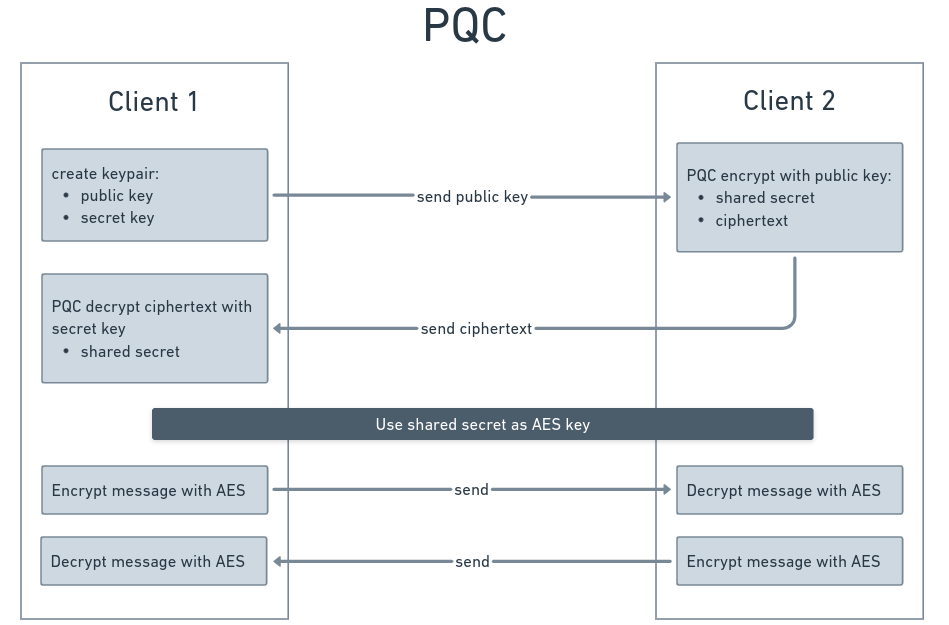
\includegraphics[width=1\linewidth]{resources/PQC_Diagram.png}
	\caption{Workflow}
	\label{fig:pqcdiagram}
\end{figure}

\begin{enumerate}
	\item Client 1 generates a key pair (\texttt{pqcrystals\_kyber768\_ref\_keypair}).
	\item Client 1 sends the public key to Client 2.
	\item Client 2 encapsulates a secret (\texttt{pqcrystals\_kyber768\_ref\_enc}), generating a ciphertext (1088 bytes) and a shared secret.
	\item Client 2 sends the ciphertext to Client 1.
	\item Client 1 decapsulates the ciphertext (\texttt{pqcrystals\_kyber768\_ref\_dec}), recovering the shared secret.
\end{enumerate}

Now Client 1 and Client 2 have the same shared secret, which can be used as a key for symmetic encryption. As the shared secret in Kyber is 32 bytes, we use AES-256.\\

% Thus, we have a hybrid system, combining the post-quantum secure CRYSTALS-KYBER with the pre-quantum algorithm AES-256.


\section{Testing}
To test the connections during development, we used Pidgin \cite{pidginwebsite2023}. Pidgin is a chat program which lets you log into accounts on multiple chat networks simultaneously. It is compatible with XMPP, so we were able to send a message from one onion address to another one.\\

For the ultimate test of qChat's capabilities, we successfully conducted a direct message exchange between our computers.

\section {Security Layers}


\begin{figure}[H]
	\centering
	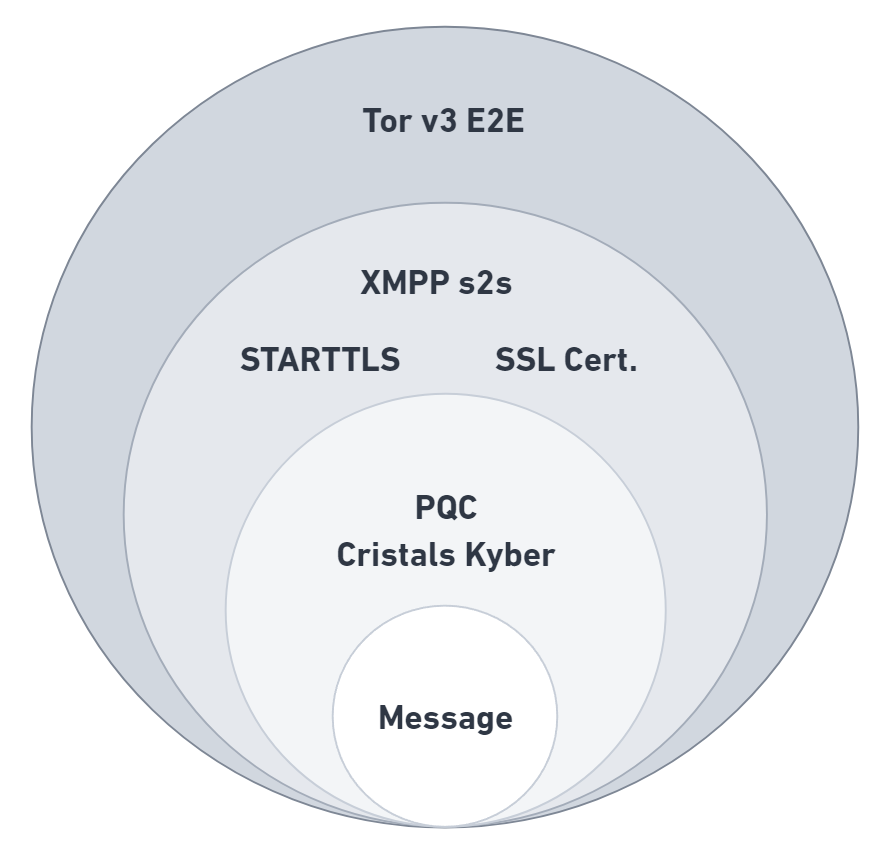
\includegraphics[width=0.7\linewidth]{resources/securitylayers.png}
	\caption{Security Layers}
	\label{fig:securitylayers}
\end{figure}

First, the message is encrypted using AES-256. The symmetric key was initially negotiated in the key exchange \ref{fig:pqcdiagram} with the Kyber PQC algorithm, which enhances confidentiality by protecting it from future quantum computer threats.\\ \\
After securing the message with Kyber, the XMPP server initiates a TLS (Transport Layer Security) session to further encrypt the message. The TLS layer not only adds another level of confidentiality, but also contributes to integrity by ensuring that the data is not tampered with during transmission. The server uses a Secure Socket Layer (SSL) certificate for authentication, confirming the identity of the communicating parties and protecting against man-in-the-middle attacks. \\ \\
Once the TLS session is established, the XMPP server sends the encrypted message through the Tor network. We use Tor version 3, which enhances privacy and anonymity, key aspects of confidentiality. This layer ensures that the identity of the communicating parties and the route of the data transmission are concealed. Tor uses Distributed Hash Tables (DHT) to improve availability. In a DHT system, data is distributed across a network of nodes, meaning there is no single point of failure. \\ \\
This combination of PQC, TLS, and Tor v3 provides a robust security model that aims to protect against a wide range of potential threats. \\

